\documentclass{article}
\usepackage{amsmath,amsfonts,amsthm,amssymb,amsopn,bm}
\usepackage[margin=.9in]{geometry}
\usepackage{graphicx}
\usepackage{url}
\usepackage[usenames,dvipsnames]{color}
\usepackage{fancyhdr}
\usepackage{multirow}
\usepackage{listings}
\usepackage{hyperref}
\usepackage{subfig}

\definecolor{keywords}{RGB}{255,0,90}
\definecolor{comments}{RGB}{0,0,113}
\definecolor{red}{RGB}{160,0,0}
\definecolor{green}{RGB}{0,150,0}
 
\lstset{language=Python, 
        basicstyle=\ttfamily\tiny, 
        keywordstyle=\color{keywords},
        commentstyle=\color{comments},
        stringstyle=\color{red},
        showstringspaces=false}

\newcommand{\argmax}{\arg\!\max}
\newcommand{\argmin}{\arg\!\min}
\newcommand{\field}[1]{\mathbb{#1}}
\newcommand{\1}{\mathbf{1}}
\newcommand{\E}{\mathbb{E}} 
\renewcommand{\P}{\mathbb{P}}
\newcommand{\N}{\mathcal{N}} % NormalDist
\newcommand{\R}{\field{R}} % real domain
% \newcommand{\C}{\field{C}} % complex domain
\newcommand{\F}{\field{F}} % functional domain
\newcommand{\T}{^{\textrm T}} % transpose
\def\diag{\text{diag}}

%% operator in linear algebra, functional analysis
\newcommand{\inner}[2]{#1\cdot #2}
\newcommand{\norm}[1]{\left\|#1\right\|}
\newcommand{\twonorm}[1]{\|#1\|_2^2}
% operator in functions, maps such as M: domain1 --> domain 2
\newcommand{\Map}[1]{\mathcal{#1}}
\renewcommand{\theenumi}{\alph{enumi}} 

\newcommand{\Perp}{\perp \! \! \! \perp}

\newcommand\independent{\protect\mathpalette{\protect\independenT}{\perp}}
\def\independenT#1#2{\mathrel{\rlap{$#1#2$}\mkern2mu{#1#2}}}
\newcommand{\vct}[1]{\boldsymbol{#1}} % vector
\newcommand{\mat}[1]{\boldsymbol{#1}} % matrix
\newcommand{\cst}[1]{\mathsf{#1}} % constant
\newcommand{\ProbOpr}[1]{\mathbb{#1}}
\newcommand{\points}[1]{\small\textcolor{magenta}{\emph{[#1 points]}} \normalsize}
\date{{}}

\setlength\parindent{0px}

\begin{document}
\title{Homework \#3 A}
\author{\normalsize{Spring 2020, CSE 446/546: Machine Learning}\\
\normalsize{Dino Bektesevic}}
\maketitle

Collaborated: Conor Sayers, Joachim Moeyenes, Jessica Birky, Leah Fulmer

\section*{Conceptual Questions}
A1. The answers to these questions should be answerable without referring to external materials.  Briefly justify your answers with a few word
\begin{enumerate}
\item \points{2} True or False: Given a data matrix $X\in \R^{n\times d}$ where $d$is much smaller than $n$, if we project our data onto a $k$ dimensional subspace using PCA where $k=\text{rank} X$, our projection will have 0 reconstruction error (we find a perfect representation of our data, with no information loss)

\item \points{2} True or False: The maximum margin decision boundaries that support vector machines construct have the lowest generalization error among all linear classifiers.

\item \points{2} True or False: An individual observation $x_i$ can occur multiple times in a single bootstrap sample from a dataset $X$, even if $x_i$ only occurs once in $X$.

\item \points{2} True or False: Suppose that the SVD of a square $n\times n$ matrix $X$ is $USV^T$, where $S$ is a diagonal $n\times n$ matrix. Then the rows of $V$ are equal to the eigenvectors of $X^TX$.

\item \points{2} True or False: Performing PCA to reduce the feature dimensionality and then applying the Lasso results in an interpretable linear model.

\item \points{2} True or False: choosing $k$ to minimize the k-means objective (see Equation (1) below) is a good way to find meaningful clusters.

\item \points{2} Say you trained an SVM classifier with an RBF kernel ($K(u,v) = \exp(\frac{-||u-v||^2_2}{ 2\sigma^2}$)). It seems to under-fit the training set: should you increase or decrease $\sigma$?
\end{enumerate}


\newpage
\section*{Kernels and the Bootstrap}
A2.\points{5} Suppose that our inputs $x$ are one-dimensional and that our feature map is infinite-dimensional: $\psi(x)$ is a vector whose $i$-th component is 
$$\frac{1}{\sqrt{i!}}e^{\frac{-x^2}{2}}x^i$$
for all nonnegative integers $i$. (Thus, $\psi$ is an infinite-dimensional vector.) Show that $K(x,x') =e^{-1/2(x-x')^2}$ is a kernel function for this feature map, i.e., $\psi(x)\cdot \psi(x') = e^{-1/2(x-x')^2}$. Hint:Use the Taylor expansion of $e$. (This is the one dimensional version of the Gaussian (RBF) kernel).


\newpage
A3. This problem will get you familiar with kernel ridge regression using the polynomial and RBF kernels. First, let’s generate some data. Let $n=30$ and $f_*(x)=4\sin(\pi x)\cos(6\pi x^2)$. For $i= 1,\hdots,n$ let each $x_i$ be drawn uniformly at random on $[0,1]$ and $y_i=f_*(x_i) + i$ where $i\approx\N(0,1)$. For any function $f$, the true error and the train error are respectively defined as 
$$\varepsilon_{\text{true}} (f) = E_{XY} [(f(X)-Y)^2]$$
$$\varepsilon_{\text{train}} (f) =\frac{1}{n}\sum_{i=1}^n = (f(x_i) - y_i)$$
Using kernel ridge regression, construct a predictor 
$$\alpha = \argmin_\alpha ||K\alpha - y||^2 + \lambda\alpha^TK\alpha$$
$$\hat f(x) = n\sum_{i=1}^k \widehat\alpha_i k(x_i,x)$$
where $K_{i,j}=k(x_i,x_j)$ is a kernel evaluation and $\lambda$ is the regularization constant. Include any code you use for your experiments in your submission.
\begin{enumerate}
    \item \points{10} Using leave-one-out cross validation, find a good $\lambda$and hyperparameter settings for the following kernels:
    \begin{enumerate}
        \item $k_{poly}(x,z) = (1 +x^Tz)^d$ where $d\in\N$ is a hyperparameter,
        \item $k_{rbf}(x,z) = \exp(-\gamma ||x-z||^2$ where $\gamma>0$ is a hyperparameter,
    \end{enumerate} Report the values of $d$,$\gamma$, and the $\lambda$ values for both kernels.\\
    
    For RBF kernel I find optimal lambda: 0.07757, gamma: 141.9 sampled \@ minimal error: 1.603 (log(err)=0.4717). \\
    For polynomial kernel I find optimal lambda: 0.8221, degree: 48.0 sampled \@ minimal error: 1.87 (log(err)=0.626). 
    \begin{figure}[h!]
        \centering 
        \subfloat[]{{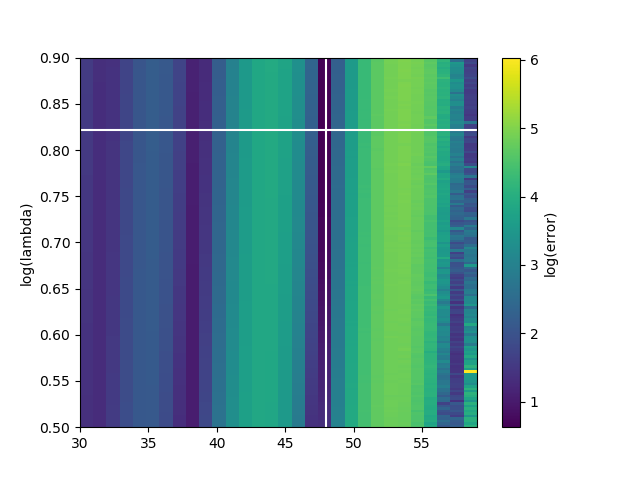
\includegraphics[width=0.47\textwidth]{HW3/HW3_plots/A3a_PolyFit.png} }}
        \subfloat[]{{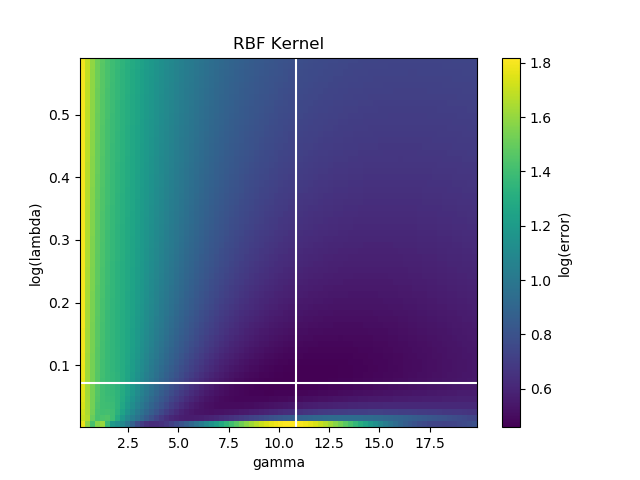
\includegraphics[width=0.47\textwidth]{HW3/HW3_plots/A3a_RBFFit.png} }}
        \caption{Cross validated error sampled at different pairs of regularization (y-axis) and hyper (x-axis) parameters. White cross marks the minimal sampled cross validation error.}
    \end{figure}


    \newpage
    \item \points{10} Let $\widehat f_{\text{poly}}(x)$ and $\widehat f_{\text{rbf}} (x)$ be the functions learned using the hyperparameters you found in part a. For a single plot per function $\widehat f\in \{\widehat f_{\text{poly}}(x), \widehat f_{\text{poly}}(x)\}$, plot the original data $\{(x_i,y_i)\}^n_{i=1}$, the true $f(x)$,and $\widehat f(x)$ (i.e., define a fine grid on $[0,1]$ to plot the functions). 
    \begin{figure}[h!]
    \centering 
        \subfloat[]{{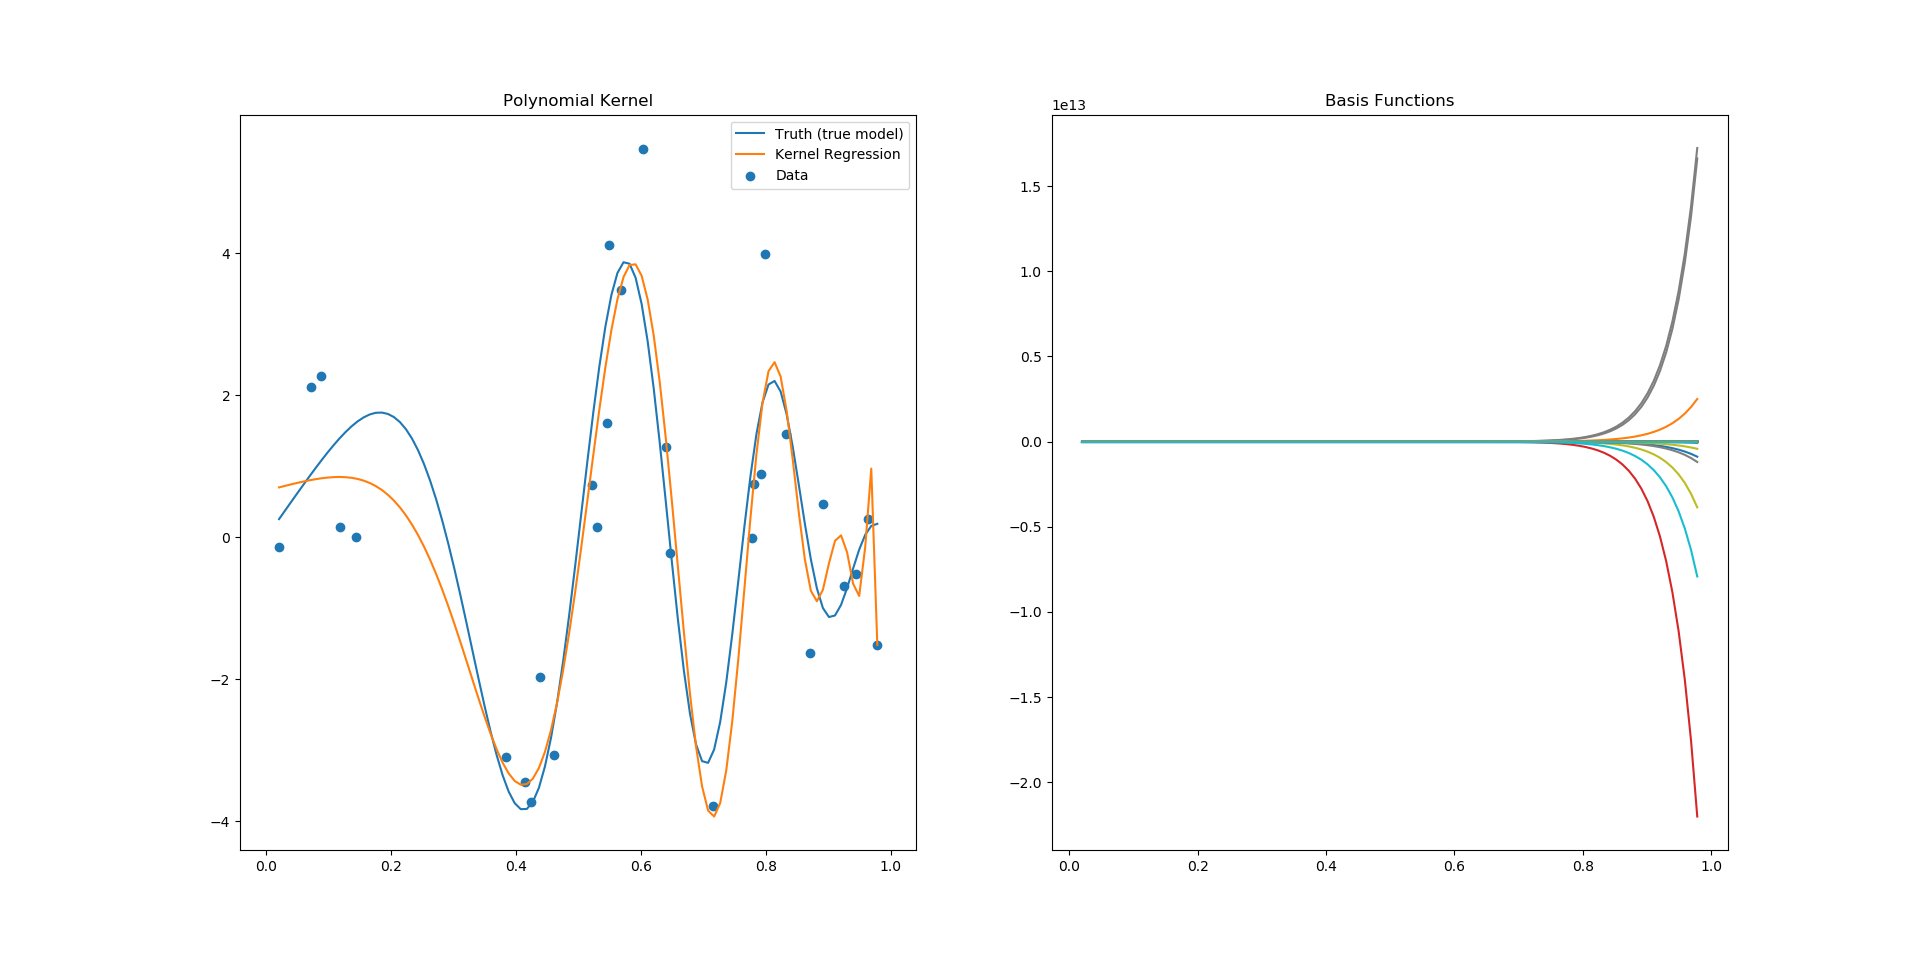
\includegraphics[width=0.47\textwidth]{HW3/HW3_plots/A3b_PolyBasis.png} }}
        \subfloat[]{{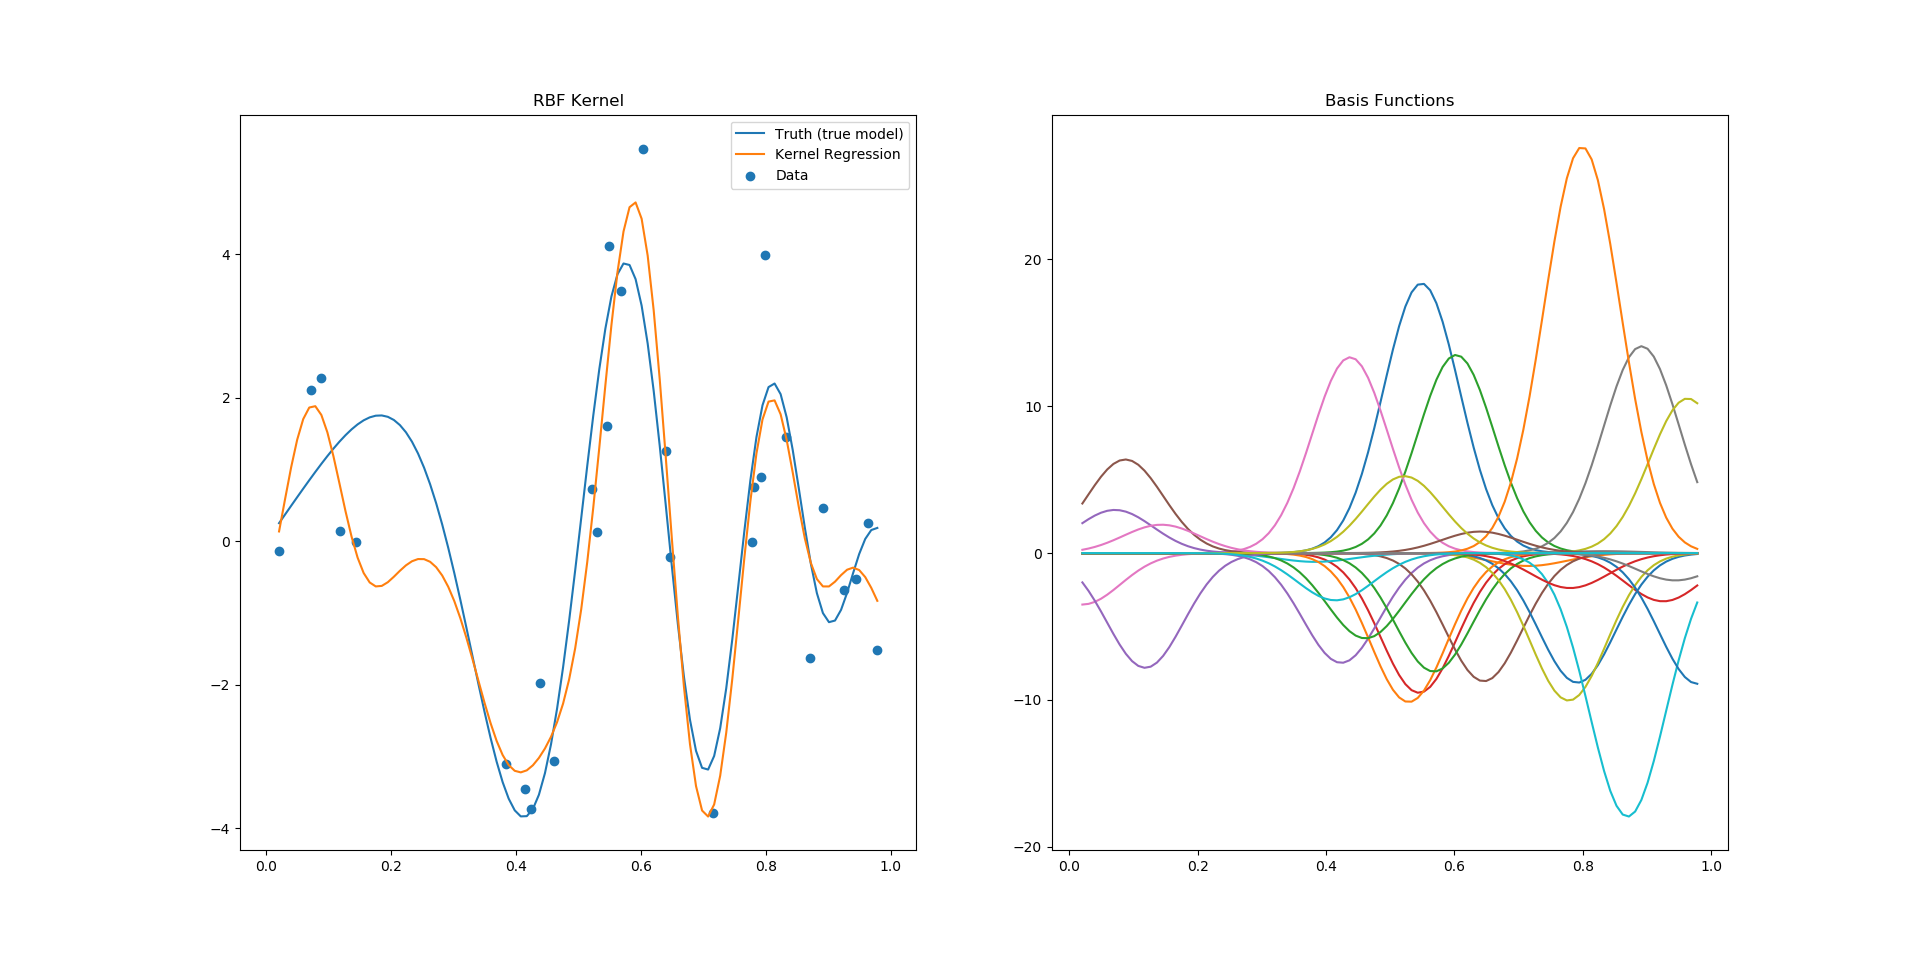
\includegraphics[width=0.47\textwidth]{HW3/HW3_plots/A3b_RBFBasis.png} }}
        \caption{Kernels evaluated on [0,1] using the best fit values of regularization and hyper parameters.}
    \end{figure}
    
    \newpage
    \item \points{5} We wish to build bootstrap percentile confidence intervals for $\widehat f_{\text{poly}}(x)$ and $\widehat f_{\text{rbf}}(x)$ for all $x\in[0,1]$ from part b. Use the non-parametric bootstrap with $B=300$ bootstrap iterations to find 5\% and 95\% percentiles at each point $x$ on a fine grid over $[0,1]$. 
    
    Specifically, for each bootstrap sample $b\in\{1,...,B\}$, draw uniformly at randomly with replacement $n$ samples from $\{(x_i,y_i)\}^n_{i=1}$, train an $\widehat f_n$ using the $b$-th resampled dataset, compute $\widehat f_b(x)$ for each $x$ in your fine grid; let the 5th percentile at point $x$ be the largest value $\nu$ such that $B\sum^B_{b=1} \1\{\widehat f_b (x) \leq \nu \} leq .05$, define the 95\% analogously. Plot the 5 and 95 percentile curves on the plots from part b.
    \begin{figure}[h!]
    \centering 
        \subfloat[]{{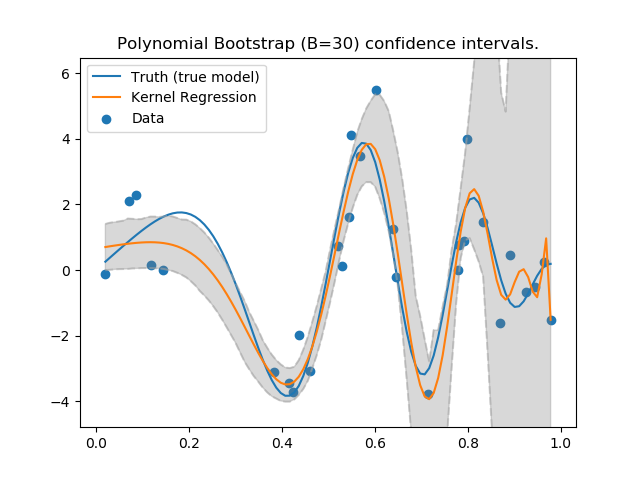
\includegraphics[width=0.47\textwidth]{HW3/HW3_plots/A3c_PolyBootstrapCI.png} }}
        \subfloat[]{{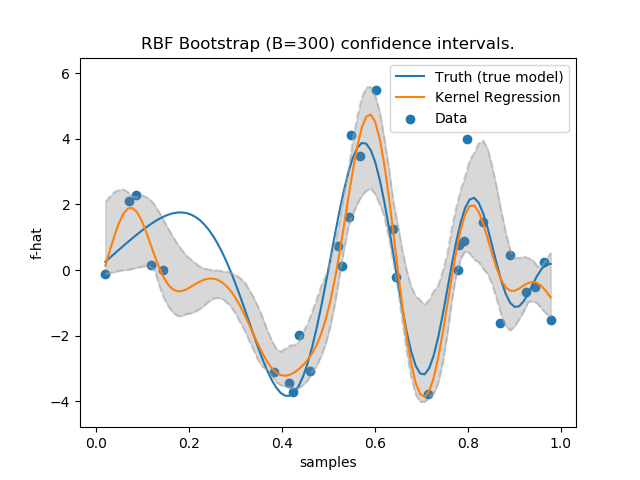
\includegraphics[width=0.47\textwidth]{HW3/HW3_plots/A3c_RBFBootstrapCI.png} }}
        \caption{Bootstrapped 5th and 95th percentile confidence interval.}
    \end{figure}
    
    
    \item \points{5} Repeat parts a, b, and c with $n=300$, but use 10-fold CV instead of leave-one-out for part a.
    
    \item \points{5}For this problem, use the $\widehat f_{\text{poly}}$ and $\widehat f_{\text{rbf}}$ learned in part d. Suppose $m=1000$ additional samples $(x'_1,y'_1),\hdots ,(x'_m,y'_m)$ are drawn i.i.d. the same way the first $n$ samples were drawn. Use the non-parametric bootstrap with $B=300$ to construct a confidence interval on $E[(Y - \widehat f_{\text{poly}} (X))^2 - (Y - \widehat f_{\text{rbf}})^2]$ (i.e. randomly draw with replacement $m$ samples denoted as $\{(\tilde x'_i, \tilde y'_i)\}^m_{i=1}$ from $\{(\tilde x'_i, \tilde y'_i)\}^m_{i=1}$ and compute 
    $$\frac{1}{m}\sum^m_{i=1} ((\tilde  y'_i - \widehat f_{\text{poly}} (\tilde x'_i))^2 - (\tilde y'_i - ]widehat f_{\text{rbf}} (\tilde x'_i))^2)$$
    repeat this $B$ times) and find 5\% and 95\% percentiles. Report these values.Using this confidence interval, is there statistically significant evidence to suggest that one of $\widehat f_{\text{poly}}$ $\widehat f_{\text{rbf}}$ is better than the other at predicting $Y$ from $X$? (Hint:  does the confidence interval contain 0?)
\end{enumerate}


\newpage
\section*{$k$-means clustering}
A4. Given a dataset $x_1,\hdots, x_n \in\R^d$ and an integer $1\leq k \leq n$, recall the following $k$-means objective function 
$$\min_{pi_1,\hdots,\pi_k} \sum_{i=1}^k\sum_{j\in\pi_i} ||x_j-\mu_i||^2_2$$
$$\mu_i=\frac{1}{\pi_i} \sum_{j\in\pi_i} x_j$$
Above, $\{\pi_i\}^k_{i=1}$ is a partition of $\{1,2,\hdots,n\}$. The objective is NP-hard to find a global minimizer of. Nevertheless Lloyd’s algorithm, the commonly-used heuristic which we discussed in lecture, typically works well in practice.
\begin{enumerate}
    \item \points{5} Implement Lloyd’s algorithm for solving the $k$-means objective. Do not use any off-the-shelf implementations, such as those found in scikit-learn.  Include your code in your submission.
    \item \points{5} Run the algorithm on the training dataset of MNIST with k=10, plotting the objective function as a function of the iteration number. Visualize (and include in your report) the cluster centers as a28$\times$28 image.
    \item \points{5} Fork=$\{2,4,8,16,32,64\}$ run the algorithm on the training dataset to obtain centers $\{\mu_i\}^k_{i=1}$. If $\{(x_i,y_i)\}^n_{i=1}$ and $\{(x'_i,y'_i)\}^m_{i=1}$ denote the training and test sets, respectively, plot the training error $\frac{1}{n}\sum^n_{i=1}\min_{j=1,\hdots,k} ||\mu_j - x_i ||^2_2$ and test error $\frac{1}{m}\sum^m_{i=1} \min_{j=1,\hdots,k} ||\mu_j - x'_i||^2_2$ as a function of $k$ on the same plot.
\end{enumerate}


\newpage
\section*{Neural Networks for MNIST}
A5. In Homework 1, we used ridge regression for training a classifier for the MNIST data set. Students who did problem B.2 also used a random feature transform. In Homework 2, we used logistic regression to distinguish between the digits 2 and 7. Students who did problem B.4 extended this idea to multinomial logistic regression to distinguish between all 10 digits. In this problem, we will use PyTorch to build a simple neural network classifier for MNIST to further improve our accuracy. We will implement two different architectures: a shallow but wide network, and a narrow but deeper network. For both architectures, we used to refer to the number of input features (in MNIST, $d=28^2=784$), $h_i$ to refer to the dimension of the $i$-th hidden layer and $k$ for the number of target classes (in MNIST, $k=10$).For the non-linear activation, use ReLU. Recall from lecture that
$$ReLU(x) = \begin{cases} 
    x &\mbox{if } x \geq 0\\
    0 &\mbox{if } x < 0 \\
\end{cases} $$


\textbf{Weight Initialization}

Consider a weight matrix $W\in\R^{n\times m}$ and $b\in\R^n$. Note that here $m$ refers to the input dimension and $n$ to the output dimension of the transformation $Wx+b$. Define $\alpha = 1/\sqrt m$. Initialize all your weight matrices and biases according to $Unif(-\alpha,\alpha)$.

\textbf{Training} 

For this assignment, use the Adam optimizer from torch.optim. Adam is a more advanced form of gradient descent that combines momentum and learning rate scaling. It often  converges faster than regular gradient descent. You can use either Gradient Descent or any form of Stochastic Gradient Descent. Note that you are still using Adam,  but might pass either the full data, a single datapoint or a batch of data to it. Use cross entropy for the loss function and ReLU for the non-linearity.


\textbf{Implementing the Neural Networks}
\begin{enumerate}
    \item \points{10} Let $W_0\in\R^{h\times d}$, $b_0\in\R^h$, $W_1\in\R^{k\times h}$, $b_1\in\R^k$ and $\sigma (z): \R \rightarrow \R$ some non-linear activation function. Given some $x\in\R^d$, the forward pass of the wide, shallow network can be formulated as:
    $$\F_1(x) = W_1\sigma (W_0x+b_0) + b+1$$
    Use $h=64$ for the number of hidden units and choose an appropriate learning rate. Train the network until it reaches 99\% accuracy on the training data and provide a training plot (loss vs. epoch). Finally evaluate the model on the test data and report both the accuracy and the loss.
    
    \item \points{10} Let $W_0\in\R^{h_0\times d}$, $b_0\in\R^{h_0}$, $W_1\in\R^{h_1\times h_0}$, $b_1 \in \R^{h_1}$, $W_2\in \R^{k\times h_2}$, $b_2 \in \R^k$ and $\sigma (z): \R \rightarrow \R$ some non-linear activation function. Given some $x\in\R^d$, the forward pass of the network can be formulated as:
    $$\F_2(x) = W_2\sigma(W_1\sigma (W_0x + b_0) +b_1) + b_2$$
    Use $h_0 = h_1= 32$ and perform the same steps as in part a.
    
     \item \points{5} Compute the total number of parameters of each network and report them. Then compare the number of parameters as well as the test accuracies the networks achieved. Is one of the approaches (wide,shallow vs narrow, deeper) better than the other? Give an intuition for why or why not.
\end{enumerate}

\newpage
\section*{PCA}

Let’s do PCA on MNIST dataset and reconstruct the digits in the dimensionality-reduced PCA basis. You will actually compute your PCA basis using the training dataset only, and evaluate the quality of the basis on the  test set, similar to the k-means reconstructions of above. Because 50,000 training examples are size $28\times 28$ so begin by flattening each example to a vector to obtain $X_{\text{train}} \in \R^{50,000 \times d}$ and $X_{\text{test}} \in \R^{10,000\times d}$ for $d:=784$

A6. Let $\mu\in\R^d$ denote the average of the training examples in $X_{\text{train}}$, i.e., $\mu = \frac{1}{d} X^T_{\text{train}}$. Now let $\sum (X_{\text{train}} - \1 \mu^T)^T (X_{\text{train}} - \1\mu^T)/50000$ denote the sample covariance matrix of the training examples, and let $\sum =UDU^T$ denote the eigenvalue decomposition of $\sum$
\begin{enumerate}
    \item \points{2} If $\lambda_i$ denotes the $i-th$ largest eigenvalue of $\sum$, what are the eigenvalues $\lambda_1, \lambda_2, \lambda_{10}, \lambda_{30}$, and $\lambda_{50}$? What is the sum of eigenvalues $\sum^d_{i=1}\lambda_i$?
    
    \item \points{5} Any example $x\in\R^d$ (including those from either the training or test set) can be approximated using just $\mu$ and the first $k$ eigenvalue, eigenvector pairs, for any $k=1,2,\hdots,d$.  For any k, provide a formula for computing this approximation.
    
    \item \points{5} Using this approximation, plot the reconstruction error from $k=1$ to 100 (the X-axis is $k$ and the Y-axis is the mean-squared error reconstruction error) on the training set and the test set (using the $\mu$ and the basis learned from the training set). On a separate plot, plot 
    $$1 - \frac{\sum^k_{i=1}\lambda_i}{\sum^d_{i=1}\lambda_i}$$
    from $k=1$ to 100.
    
    \item \points{3} Now let us get a sense of what the top PCA directions are capturing. Display the first  10 eigenvectors as images, and provide a brief interpretation of what you think they capture.
    
    \item \points{3} Finally, visualize a set of reconstructed digits from the training set for different values of $k$. In particular provide the reconstructions for digits 2,6,7 with values $k=5,15,40,100$ (just choose an image from each digit arbitrarily). Show the original image side-by-side with its reconstruction.  Provide a brief interpretation, in terms of your perceptions of the quality of these reconstructions and the dimensionality you used.
\end{enumerate}

\end{document}
